% ==============================================================================
% 插曲 5：计算开销 (Intermezzo 5: The Cost of Computation)
% ==============================================================================

\intermezzo{插曲 5：计算开销}
\label{sec:intermezzo05}

当程序 $f$ 顺利通过以下三项测试时，你能断言关于 $f$ 的哪些性质？

\begin{lstlisting}[language=BSL]
(check-expect (f 0) 0)
(check-expect (f 1) 1)
(check-expect (f 2) 8)
\end{lstlisting}

如果这道题出现在标准测试卷中，你可能会自然写出立方函数：
\begin{lstlisting}[language=BSL]
(define (f x) (expt x 3))
\end{lstlisting}
但事实上，没有任何理由能排除如下定义：
\begin{lstlisting}[language=BSL]
(define (f x) (if (= x 2) 8 (* x x)))
\end{lstlisting}
测试仅仅表明：程序在\textbf{某些特定输入}上的行为符合预期，仅此而已。

同理，对特定输入测试程序的求值耗时，仅仅告诉你针对这些孤立输入的执行时间——它无法外推到未知规模的输入。设想你有两个程序：\code{prog-linear} 与 \code{prog-square}，它们在给定相同输入时总是产生相同的答案，且在你随手挑选的若干测试样本上，\code{prog-linear} 总是比 \code{prog-square} 更快。第 26.4 节便展示了这样一对程序：结构型递归的 \code{gcd-structural} 与生成型递归的 \code{gcd-generative}，后者实测耗时远短于前者。

你有多大把握能断言 \code{prog-linear} 在任何情况下都优于 \code{prog-square}？考察图~\ref{fig:runtime-crossover} 中的函数曲线图。横轴表示输入规模（例如列表的长度 $n$），纵轴表示计算耗时。直线代表 \code{prog-linear} 的耗时，而抛物曲线代表 \code{prog-square} 的耗时。在阴影区域内，由于常数因子的影响，\code{prog-linear} 的耗时反而高于 \code{prog-square}；直到跨过交叉点阈值之后，\code{prog-square} 的耗时才发生剧烈陡增并远超 \code{prog-linear}。如果你仅仅在阴影区域的小规模输入上测试性能，而用户实际运行的数据却大量处于非阴影的大规模区域，你就会向用户交付一个错误且低效的程序。

\begin{figure}[htbp]
  \centering
  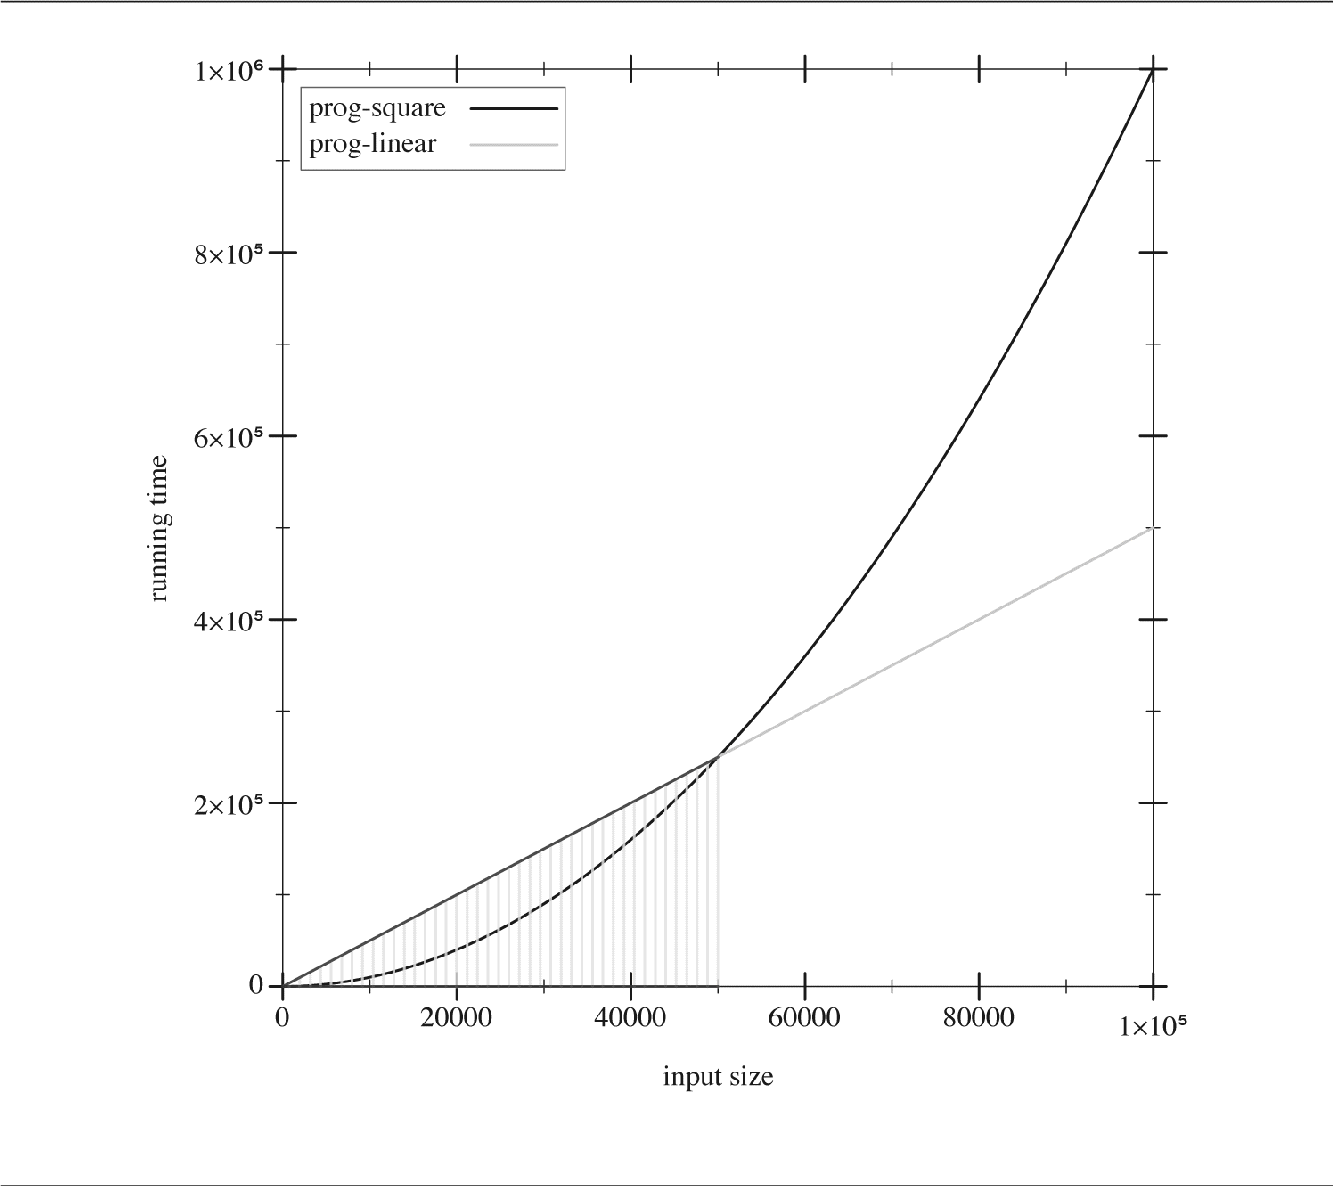
\includegraphics[width=0.75\textwidth]{images/00685.png}
  \caption{两种运行时间表达式的增长对比与交叉平衡点}
  \label{fig:runtime-crossover}
\end{figure}

本插曲正式引入\term{算法分析（algorithmic analysis）}的核心思想。它使程序员能够超越机器与环境的偶然干扰，对程序的性能本质做出普遍性陈述。任何严谨的计算机科学家与软件工程师都必须彻底精通这一概念。

\intermezzosection{具体时间与抽象时间}

第 26.4 节指出，\code{gcd-generative} 之所以从根本上优于 \code{gcd-structural}，是因为前者求解时所需的\textbf{递归步骤总数}远少于后者。以此为起点，我们来分析第 9 章中计算列表长度的简单程序 \code{how-many}：

\begin{lstlisting}[language=BSL]
(define (how-many a-list)
  (cond
    [(empty? a-list) 0]
    [else (+ (how-many (rest a-list)) 1)]))
\end{lstlisting}

利用插曲 1 中的代数代换规则，观察其在非空列表上的单步演算：
\begin{lstlisting}[language=BSL]
  (how-many some-non-empty-list)
== (cond
     [(empty? some-non-empty-list) 0]
     [else (+ (how-many (rest some-non-empty-list)) 1)])
== (cond
     [#false 0]
     [else (+ (how-many (rest some-non-empty-list)) 1)])
== (+ (how-many (rest some-non-empty-list)) 1)
\end{lstlisting}

在现代计算机体系中，判断列表构造器类型（\code{empty?}）、检查 \code{cond} 分支以及提取子结构（\code{rest}）所耗费的时间都是极其微小且恒定的常数。因此，\code{(how-many a-list)} 的总计算耗时，本质上正比于递归调用的总次数——对于长度为 $n$ 的列表，程序精确执行 $n$ 次递归展开。

这种抽象抽离了硬件时钟频率、编译器优化等底层偶然细节，将性能刻画为\textbf{输入规模 $n$ 与所需基本操作（递归步数）之间的函数关系}。计算机科学家称之为程序的\term{抽象运行时间（abstract running time）}。

对于 \code{how-many}，我们说它的计算时间“与输入规模 $n$ 处于同一数量级”（on the order of $n$ steps）。

并非所有程序的求值步数都像 \code{how-many} 那样固定。考察检索列表中是否包含特定符号的函数：
\begin{lstlisting}[language=BSL]
(define (contains-flatt? lo-names)
  (cond
    [(empty? lo-names) #false]
    [(cons? lo-names)
     (or (symbol=? (first lo-names) 'flatt)
         (contains-flatt? (rest lo-names)))]))
\end{lstlisting}

若目标元素恰好位于列表首位，只需 0 次递归即可立即返回；而若目标元素位于列表末尾或根本不存在，则必须完整遍历所有 $n$ 个元素。这一差异引出了算法分析的三种核心视角：
\begin{itemize}
  \item \textbf{最好情况分析（Best-case analysis）}：针对最有利于程序的输入形态评估性能（例如首元素即为目标，耗时为常数步）。
  \item \textbf{最坏情况分析（Worst-case analysis）}：针对最苛刻极端、最耗时的输入评估性能瓶颈（例如目标位于末尾，需遍历 $n$ 步）。
  \item \textbf{平均情况分析（Average-case analysis）}：假设输入数据随机均匀分布，评估平均期望耗时（例如平均在中间位置找到目标，需 $n/2$ 步）。
\end{itemize}

在抽象分析中，常数因子（如 $n/2$ 中的系数 $1/2$）可以被忽略。设每步基本操作耗时为常数 $k$，换用两倍主频的新 CPU 后耗时减半为 $k/2$；但无论系数常数如何变化，增长的几何本质始终是 $n$ 的线性函数。

现在考察插入排序算法（第 11 章）。对其进行手工推演：
\begin{lstlisting}[language=BSL]
  (sort (list 3 1 2))
== (insert 3 (sort (list 1 2)))
== (insert 3 (insert 1 (sort (list 2))))
== (insert 3 (insert 1 (insert 2 (sort '()))))
== (insert 3 (insert 1 (insert 2 '())))
== (insert 3 (insert 1 (list 2)))
== (insert 3 (list 2 1))
== (list 3 2 1)
\end{lstlisting}

\code{sort} 首先递归展开 $n$ 次，随后触发 $n$ 次 \code{insert} 插入操作。每次将元素插入到长度为 $l$ 的有序列表时，平均需要比较 $l/2$ 次。对于长度为 $n$ 的列表，插入操作的平均总步数为：
\[ \sum_{i=1}^{n-1} \frac{i}{2} = \frac{1}{2} \cdot \frac{n(n-1)}{2} = \frac{1}{4} n^2 - \frac{1}{4} n \]
当 $n$ 增长时，$n^2$ 项起决定性支配作用。因此，插入排序算法的耗时“与 $n^2$ 处于同一数量级”。

最后考察第 16.2 节中寻找列表最小值的朴素实现 \code{inf}：
\begin{lstlisting}[language=BSL]
(define (inf l)
  (cond
    [(empty? (rest l)) (first l)]
    [else (if (< (first l) (inf (rest l)))
              (first l)
              (inf (rest l)))]))
\end{lstlisting}
当列表按降序排列时（最坏情况），\code{if} 的判断条件为假，程序被迫在 \code{else} 分支中再次对 \code{(rest l)} 重新完整执行一次递归调用！对于包含 4 个元素的列表，需要执行 8 次调用；每增加一个元素，调用树的分支数直接翻倍。其总递归步数为 $2^{n-1}$，属于灾难性的\textbf{指数级复杂度}（$O(2^n)$）。

\begin{exercise}{局部变量优化 infL 的复杂度分析}{484}\label{ex:484}
回顾利用 \code{local} 避免重复计算的改进版本 \code{infL}：
\begin{lstlisting}[language=BSL]
(define (infL l)
  (cond
    [(empty? (rest l)) (first l)]
    [else (local ((define s (infL (rest l))))
            (if (< (first l) s) (first l) s))]))
\end{lstlisting}
推导对 \code{(list 3 2 1 0)} 的求值过程。论证在最好与最坏情况下，\code{infL} 的步数均已降为 $n$ 数量级。
\end{exercise}

\begin{exercise}{数字二叉树求和 sum-tree}{485}\label{ex:485}
数字树（Number Tree）要么是一个数字，要么是一对数字树构成的有序对。设计函数 \code{sum-tree} 计算树中所有数字的总和。
分析其抽象运行时间：如何合理定义一棵树的“规模”？在相同规模下，何种树形对应最坏情况？何种对应最好情况？
\end{exercise}

\intermezzosection{“大 $O$ 记号”的形式化定义}

计算机科学使用严格的数学语言——\term{大 $O$ 记号（Big-O notation）}来标准化上述关于增长数量级的讨论。

\begin{notebox}[大 $O$ 记号定义]
设 $g(n)$ 是定义在自然数集合上的函数。记号 $\mathcal{O}(g)$（读作“$g$ 的大 $O$”）表示一类函数集合。若存在正实数 $c$ 与正整数 $n_0$（即 \code{bigEnough}），使得对于所有满足 $n \ge n_0$ 的自变量 $n$，不等式恒成立：
\[ f(n) \le c \cdot g(n) \]
则称函数 $f$ 属于 $\mathcal{O}(g)$，记作 $f \in \mathcal{O}(g)$（或通俗写作 $f(n) = \mathcal{O}(g(n))$）。

\textbf{术语含义}：若 $f \in \mathcal{O}(g)$，则表明当问题规模充分大时，$f$ 的增长速度\textbf{绝不差于（不超过）} $g$ 的常数倍。
\end{notebox}

以前文提到的线性程序与平方程序为例：
\[ H(n) = 1000n, \quad G(n) = n^2 \]
选取常数 $c = 1$ 与 $n_0 = 1000$。对于任意 $n \ge 1000$，两边同乘正数 $n$ 即得：
\[ 1000n \le n^2 \implies H(n) \le 1 \cdot G(n) \]
由此在数学上严格证明了 $H \in \mathcal{O}(G)$，即线性程序从渐进意义上绝不慢于平方程序。

在大 $O$ 分析中，低阶项与常数因子均被舍弃：
\begin{itemize}
  \item $\mathcal{O}(1)$：常数复杂度，操作耗时与输入规模完全无关；
  \item $\mathcal{O}(n)$：线性复杂度，耗时与输入规模成正比；
  \item $\mathcal{O}(n \log n)$：线性对数复杂度，如快速排序的平均性能；
  \item $\mathcal{O}(n^2)$：平方复杂度，如冒泡排序、插入排序；
  \item $\mathcal{O}(2^n)$：指数复杂度，通常意味着算法对于中大规模输入完全不可用。
\end{itemize}

\begin{exercise}{证明多项式属于 O(n\textasciicircum 2)}{486}\label{ex:486}
证明函数 $f(n) = n^2 + n$ 属于 $\mathcal{O}(n^2)$。明确给出一组满足定义的常数对 $(c, n_0)$。
\end{exercise}

\begin{exercise}{指数爆炸与常数倍线性对比}{487}\label{ex:487}
考察函数 $f(n) = 2^n$ 与 $g(n) = 1000n$。证明 $g \in \mathcal{O}(f)$。如果已知现实应用中输入规模严格处于 $[3, 12]$ 之间，哪一个算法在实践中表现更优？
\end{exercise}

\begin{exercise}{对数线性与平方对比}{488}\label{ex:488}
对比函数 $f(n) = n \log_2(n)$ 与 $g(n) = n^2$。是 $f \in \mathcal{O}(g)$ 成立，还是 $g \in \mathcal{O}(f)$ 成立？写出推导依据。
\end{exercise}

\intermezzosection{为何程序应当使用结构化谓词与选择器？}

大 $O$ 分析能够从计算复杂度的角度，有力证明为什么遵循设计配方能够产出既优雅又高效的高质量程序。

考虑在数字列表中检索目标数字的任务：
\begin{lstlisting}[language=BSL]
; Number [List-of Number] -> Boolean
; 判定 x 是否存在于列表 l 中
(check-expect (search 0 '(3 2 1 0)) #true)
(check-expect (search 4 '(3 2 1 0)) #false)
\end{lstlisting}

对比以下两种实现：

\begin{figure}[htbp]
  \centering
  \begin{minipage}{0.48\textwidth}
\begin{lstlisting}[language=BSL]
(define (searchL x l)
  (cond
    [(empty? l) #false]
    [else
     (or (= (first l) x)
         (searchL x (rest l)))]))
\end{lstlisting}
  \end{minipage}
  \hfill
  \begin{minipage}{0.48\textwidth}
\begin{lstlisting}[language=BSL]
(define (searchS x l)
  (cond
    [(= (length l) 0) #false]
    [else
     (or (= (first l) x)
         (searchS x (rest l)))]))
\end{lstlisting}
  \end{minipage}
  \caption{遵循结构化谓词的 \code{searchL} 与调用长度求值的 \code{searchS}}
  \label{fig:search-comparison}
\end{figure}

左侧的 \code{searchL} 严格遵循设计配方，采用基础结构化谓词 \code{empty?} 作为条件分支。每次检查耗费 $\mathcal{O}(1)$ 常数时间，对长度为 $n$ 的列表总复杂度为严格的 $\mathcal{O}(n)$。

右侧的 \code{searchS} 脱离了配方指导，采用“先求列表长度再判断是否为 0”的直觉思路。然而在链表模型中，\code{length} 本身是一个必须从头遍历整个列表的 $\mathcal{O}(l)$ 操作！在每一次递归调用中都调用一次 \code{length}，导致总运算步数退化为：
\[ \sum_{i=1}^n i = \frac{n(n+1)}{2} \implies \mathcal{O}(n^2) \]
仅仅因为改用了一个非结构化的外部操作，程序的复杂度便硬生生从线性级堕入平方级灾难！

编写如下性能测试函数并在 DrRacket 中亲自体会这一悬殊差距：
\begin{lstlisting}[language=BSL]
; N -> [List Number Number]
; 测量 searchS 与 searchL 在长度为 n 的列表上的实际耗时
(define (timing n)
  (local ((define long-list (build-list n (lambda (i) i))))
    (list
      (time (searchS n long-list))
      (time (searchL n long-list)))))
\end{lstlisting}

在交互区分别对 $n = 10000$ 与 $n = 20000$ 执行测试：\code{searchL} 的耗时仅随 $n$ 翻倍而平缓线性翻倍，而 \code{searchS} 的耗时将呈现 4 倍的爆发式暴涨！

这一鲜明实验告诫我们：在函数设计中，\textbf{严格遵循结构化设计配方与原生谓词选择器}，不仅保证了逻辑的严谨无瑕，更为算法的底层运行性能筑起了坚不可摧的基石。
